\section{Auswertung}
\label{sec:Auswertung}
\subsection{Bestimmung der Winkelrichtgröße $D$ und des Trägheitsmoments
$I_\text{D}$ der Drillachse}
Zunächst werden die Konstanten der Apparatur, die Winkelrichtgröße $D$ und das
Eigenträgheitsmoment $I_\text{D}$ der Drillachse, bestimmt. Die Winkelrichtgröße
wird sowohl mit einer statischen Methode als auch mit einer dynamischen Methode
bestimmt, das Eigenträgheitsmoment nur mit der dynamischen Methode.

\subsubsection{statische Methode}
Mit einem Federkraftmesser wird die Rückstellkraft $F$ der Torsionsfeder bei festem
Abstand $r$ von der Drehachse in Abhängigkeit des Drehwinkels $\varphi$ gemessen.
Die Messwerte sowie die nach Gleichung (xx) berechnete Winkelrichtgröße $D$ sind
in Tabelle \ref{tab:statisch} zu aufgeführt.
\begin{table}[H]
  \centering
  \begin{tabular}{c c c c}
    \toprule
    \multicolumn{2}{c}{Drehwinkel $\varphi$} & $F$ in \si{\newton} & $D$ in \si{\newton\meter} \\
    in \si{\degree} & in \si{\radian} & & \\
    \midrule
    90  & 1.571 & 0.28 & 0.02653 \\
    100 & 1.745 & 0.30 & 0.02558 \\
    120 & 2.094 & 0.38 & 0.02700 \\
    150 & 2.618 & 0.49 & 0.02785 \\
    180 & 3.142 & 0.57 & 0.02700 \\
    200 & 3.491 & 0.61 & 0.02601 \\
    230 & 4.014 & 0.70 & 0.02595 \\
    270 & 4.712 & 0.80 & 0.02526 \\
    300 & 5.236 & 0.90 & 0.02558 \\
    330 & 5.760 & 1.00 & 0.02584 \\
    \bottomrule
  \end{tabular}
  \caption{Messwerte zur Berechnung der Winkelrichtgröße $D$ mit der statischen
  Methode.}
  \label{tab:statisch}
\end{table}
Für die Drehwinkel wird ein Ablesefehler von $\SI{5}{\degree} = \SI{0.087}{\radian}$
angenommen. Es wird der Mittelwert der Winkelrichtgröße nach Gleichung
\eqref{eqn:mittelwert} berechnet. Der Fehler ergibt sich mit Gaußscher
Fehlerfortpflanzung wie in Gleichung \eqref{eqn:fehlerfortpflanzung}. Damit ergibt
sich für die Winkelrichtgröße nach der statischen Methode
\begin{align*}
  D_\text{stat} = \SI{0.0263(3)}{\newton\meter}.
\end{align*}

\subsubsection{dynamische Methode}
Bei der dynamischen Methode wird die Schwingungsdauer $T$ für verschiedene Abstände
$a$ der Massen von der Drehachse gemessen. Die Messwerte sind in Tabelle
\ref{tab:dynamisch} dargestellt. Es wird $T^2$ gegen $a^2$ aufgetragen (siehe
Grafik \ref{fig:linreg_dynamisch}) und eine lineare Regression der Form
$y = b \cdot x + c$ mit Python durchgeführt.
\begin{figure}[H]
  \centering
  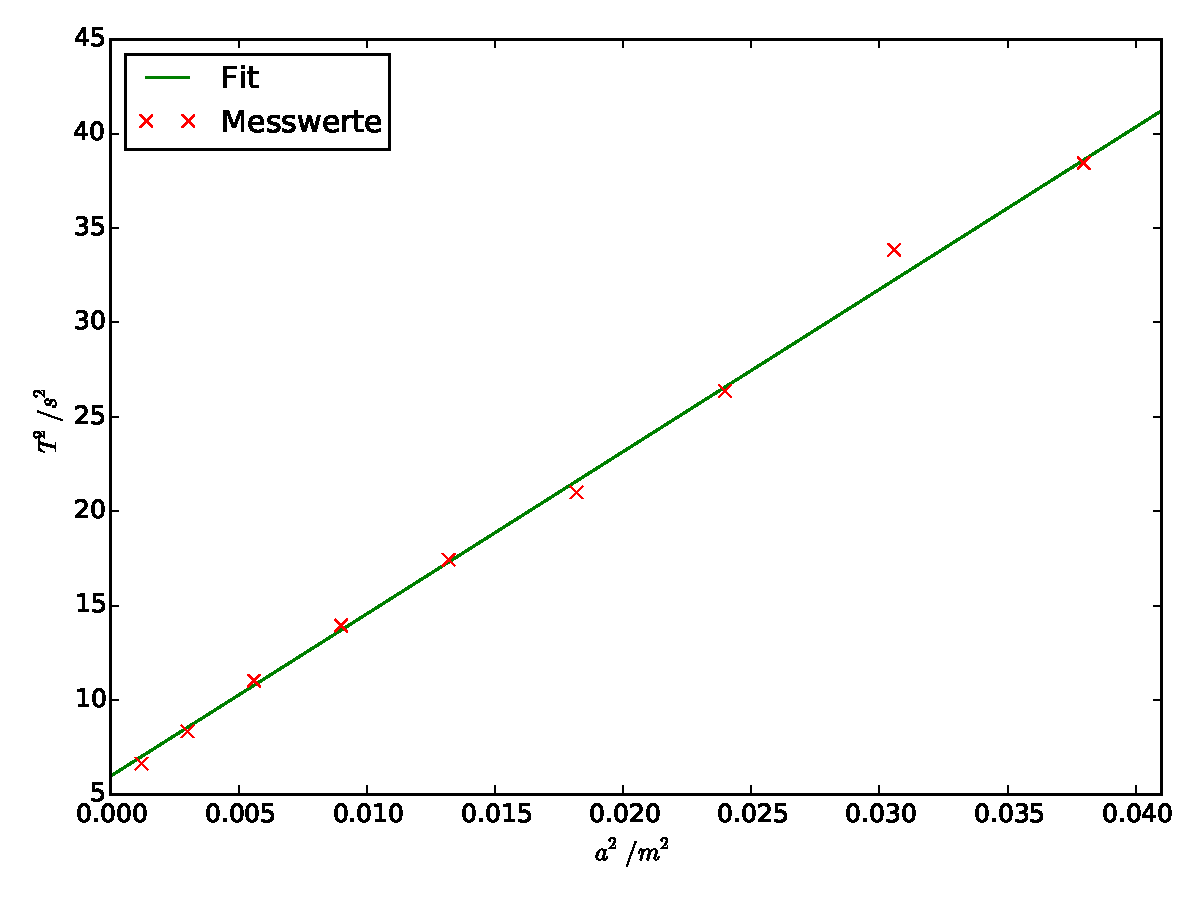
\includegraphics[width=0.8\textwidth]{dynamisch.pdf}
  \caption{Graph zur linearen Ausgleichsrechnung nach Gleichung
  \eqref{eqn:ausgleichsrechnung}.}
\end{figure}
Dies liefert mit den Messwerten aus Tabelle \ref{tab:messwerte_dynamisch} die
Parameter
\begin{align*}
  b &= \SI{860(15)}{\squared\second\per\squared\meter} \\
  c &= \SI{6.0(4)}{\squared\second}.
\end{align*}
\begin{table}
  \centering
  \begin{tabular}{c c c}
    \toprule
    Abstand $a$ in \si{\centi\meter} & \multicolumn{2}{c}{Schwingungsdauer T in \si{\second}} \\
     & 5 Perioden & 1 Periode \\
    \midrule
    3.485  & 12.87 & 2.574 \\
    5.485  & 14.44 & 2.888 \\
    7.485  & 16.60 & 3.320 \\
    9.485  & 18.67 & 3.734 \\
    11.485 & 20.87 & 4.174 \\
    13.485 & 22.91 & 4.582 \\
    15.485 & 25.67 & 5.134 \\
    17.485 & 29.09 & 5.818 \\
    19.485 & 31.00 & 6.200 \\
    21.485 & 33.53 & 6.706 \\
    \bottomrule
    \end{tabular}
  \caption{Messwerte der dynamischen Methode zur Berechnung von $D$ und
  $I_\text{D}$.}
  \label{tab:messwerte_dynamisch}
\end{table}

Die Gleichung (xx) lässt sich mit dem Gesamträgheitsmoment $I_\text{ges} =
I_\text{D} + I_\text{Z1} + I_\text{Z2}$ und den Trägheitsmomenten der Zylinder,
\begin{align*}
  I_\text{Z1} &= m_1 \left(\frac{R_1^2}{4}+\frac{h_1^2}{12}\right)+m_1 a^2 \text{ und }\\
  I_\text{Z1} &= m_2 \left(\frac{R_2^2}{4}+\frac{h_2^2}{12}\right)+m_2 a^2
\end{align*}
die um den Abstand $a$ von der Schwerpunktsachse verschoben sind, zu
\begin{align}
  T^2 &= 4 \pi^2 \frac{(m_1 + m_2)}{D} & a^2 &+ 4 \pi^2 \, \frac{m_1\left(
  \frac{R_1^2}{4} + \frac{h_1^2}{12}\right) + m_2 \left(\frac{R_2^2}{4}
  +\frac{h_2^2}{12}\right)+ I_\text{D}}{D}\\
  y &= b & x & + c
  \label{eqn:ausgleichsrechnung}
\end{align}
umformen.
Die Winkelrichtgröße wird dann mit der Gleichung
\begin{equation}
  D_\text{dyn} = 4 \pi^2 \frac{(m_1 + m_2)}{b}
  \label{eqn:D_dyn}
\end{equation}
berechnet und es ergibt sich mit Fehlerrechnung durch Python, der Steigung $b$
der linearen Regression und den Massen $m_1$ und $m_2$ aus der Tabelle
\ref{tab:gewichte}
\begin{align*}
  D_\text{dyn} = \SI{0.0205(4)}{\newton\meter}.
\end{align*}

\begin{table}
  \centering
  \begin{tabular}{c| c c}
    \toprule
        & Gewicht 1 (Zylinder) & Gewicht 2 (Zylinder)\\
    \midrule
    Masse $m$ in \si{\gram} & 223.43 & 222.50\\
    & & \\
    Durchmesser          & 3.45 & 3.46  \\
    in \si{\centi\meter} & 3.45 & 3.49  \\
                         & 3.44 & 3.48  \\
                         & 3.44 & 3.47  \\
                         & 3.45 & 3.475 \\
    & & \\
    Höhe                 & 2.97 & 2.975 \\
    in \si{\centi\meter} & 2.975 & 2.97 \\
                         & 2.97 & 2.975 \\
    \bottomrule
  \end{tabular}
  \caption{Abmessungen der zwei verwendeten Gewichte (beides Zylinder).}
  \label{tab:gewichte}
\end{table}

Das Eigenträgheitsmoment wird aus dem y-Achsenabschnitt der linearen
Ausgleichsrechnung \eqref{eqn:ausgleichsrechnung} mit der Gleichung
\begin{equation}
  I_\text{D} = m_1\left(\frac{R_1^2}{4} + \frac{h_1^2}{12}\right) + m_2 \left(
  \frac{R_2^2}{4}+\frac{h_2^2}{12}\right) - \frac{c}{b}\, (m_1 + m_2)
  \label{eqn:eigentraegheitsmoment}
\end{equation}
berechnet. Mit den Werten aus Tabelle \ref{tab:gewichte}, aus der sich insbesondere
die Radien
\begin{align*}
  R_1 &= \SI{0.01723(1)}{\meter} \text{ und }\\
  R_2 &= \SI{0.01737(3)}{\meter}
\end{align*}
und die Höhen der Zylinder
\begin{align*}
  h_1 &= \SI{0.02972(2)}{\meter} \text{ und } \\
  h_2 &= \SI{0.02973(2)}{\meter}
\end{align*}
ergeben, und den Parametern $b$ und $c$ der linearen Ausgleichsrechnung sowie
Fehlerfortpflanzung mit Python folgt für das Eigenträgheitsmoment
\begin{align*}
  I_\text{D} = \SI{-3.0(2)e-3}{\kilo\gram\squared\meter}.
\end{align*}
Ein negatives Trägheitsmoment der Drillachse ist physikalisch nicht sinnvoll,
daher wird angenommen, dass das Eigenträgheitsmoment so gering ist, dass es
in den folgenden Rechnungen vernachlässigt werden kann.

\subsection{Trägheitsmoment zweier verschiedener Körper}
Es werden die Trägheitsmomente zweier Zylinder theoretisch über die Abmessungen
und die Masse der Körper berechnet, sowie über die Schwingungsdauer bestimmt.
Der erste Zylinder (schwarz) rotiert dabei senkrecht stehend um seine
Schwerpunktsachse, der zweite Zylinder (weiß) rotiert liegend ebenfalls um seine
Schwerpunktsachse.
Die Abmessungen der Zylinder sind in Tabelle \ref{tab:abmessungen_zylinder}
dargestellt, die Messwerte der Schwingungsperiode in Tabelle
\ref{tab:messwerte_zylinder}.
\begin{table}
  \centering
  \begin{tabular}{c| c c}
    \toprule
        & Zylinder 1 & Zylinder 2 \\
    \midrule
    Masse $m$ in \si{\kilo\gram} & 1.9739 & 1.5254 \\
    & & \\
    Durchmesser          & 7.97 & 8.01  \\
    in \si{\centi\meter} & 7.94 & 8.01  \\
                         & 7.945 & 8.00  \\
    & & \\
    Höhe                 & 13.98 & 13.95 \\
    in \si{\centi\meter} & 14.01 & 13.95 \\
                         & 14.01 & 13.97 \\
    \bottomrule
  \end{tabular}
  \caption{Abmessungen der zwei Zylinder, deren Trägheitsmoment bestimmt wird.}
  \label{tab:abmessungen_zylinder}
\end{table}

\begin{table}
  \centering
  \begin{tabular}{c c c c}
    \toprule
    \multicolumn{2}{c}{Zylinder 1} & \multicolumn{2}{c}{Zylinder 2}\\
    5 $T$ in \si{\second} & 1 $T$ in \si{\second} & 5 $T$ in \si{\second} &
    1 $T$ in \si{\second} \\
    \midrule
    8.35 & 1.670 & 11.67 & 2.334 \\
    8.35 & 1.670 & 11.44 & 2.288 \\
    8.30 & 1.660 & 11.84 & 2.368 \\
    8.33 & 1.666 & 11.75 & 2.350 \\
    8.29 & 1.658 & 11.64 & 2.328 \\
    8.50 & 1.700 & 11.46 & 2.292 \\
    8.33 & 1.666 & 11.53 & 2.306 \\
    8.46 & 1.692 & 11.58 & 2.316 \\
    8.46 & 1.692 & 11.75 & 2.350 \\
    8.27 & 1.654 & 11.52 & 2.304 \\
    \midrule
    8.36 & 1.673 & 11.62 & 2.324 \\
    0.03 & 0.005 &  0.04 & 0.009 \\
    \bottomrule
  \end{tabular}
  \caption{Messwerte von fünf Perioden (5$T$) und berechnete Werte für eine Periode
  (1$T$) der zwei Zylinder. In der vorletzten Zeile stehen die Mittelwerte, in
  der letzten Zeile die Standardabweichung.}
  \label{tab:messwerte_zylinder}
\end{table}

\subsubsection{Trägheitsmoment des stehenden Zylinders}
Das Trägheitsmoment des stehenden Zylinders wird mit
\begin{equation}
  I_\text{Z,stehend} = \frac{1}{2} m_1 R_\text{Z1}^2
  \label{eqn:I_zstehend-theo}
\end{equation}
berechnet. Aus Tabelle \ref{tab:abmessungen_zylinder} ergibt sich der Radius
\begin{align*}
  R_\text{Z1} = \SI{0.03975(5)}{\meter},
\end{align*}
sodass mit den anderen Werten aus Tabelle \ref{tab:abmessungen_zylinder} und der
Gleichung \eqref{eqn:I_zstehend-theo} für das theoretisch berechnete
Trägheitsmoment des ersten Zylinders folgt:
\begin{align*}
  I_\text{Z1,theo} = \SI{1.559(4)e-3}{\squared\kilo\gram\meter}.
\end{align*}

Wird das Trägheitsmoment über die Schwingungsdauer experimentell bestimmt, so
wird die Gleichung (xx) mit dem Gesamtträgheitsmoment $I_\text{ges} = I_\text{D}
+ I_\text{Z1,exp}$ zu
\begin{equation}
  I_\text{Z1,exp} = \frac{T^2 D}{4 \pi^2} - I_\text{D}
  \label{eqn:I_zstehend-exp}
\end{equation}
mit der Mittelung der Winkelrichtgrößen
\begin{align*}
  D = \frac{D_\text{stat}+ D_\text{dyn}}{2} = \SI{0.0234(2)}{\newton\meter}
\end{align*}
umgeformt. Es ergibt sich der Wert mit der Periodendauer $T$ aus Tabelle
\ref{tab:messwerte_zylinder}
\begin{align*}
  I_\text{Z1,exp} = \SI{1.66(2)e-3}{\squared\kilo\gram\meter}.
\end{align*}
Dies entspricht einer relativen Abweichung von $\Delta I_\text{Z1} = \SI{6(1)}
{\percent}$ nach Gleichung \eqref{eqn:rel_abweichung}.


\subsubsection{Trägheitsmoment des liegenden Zylinders}
Das Trägheitsmoment des liegenden Zylinders wird mit
\begin{equation}
  I_\text{Z2,liegend} = m_2 \left(\frac{R_\text{Z2}^2}{4}
  +\frac{h_\text{Z2}^2}{12}\right)
  \label{eqn:I_zliegend-theo}
\end{equation}
berechnet. Aus Tabelle \ref{tab:abmessungen_zylinder} folgt für den Radius und
die Höhe des zweiten Zylinders
\begin{align*}
  R_\text{Z2} &= \SI{0.04003(2)}{\meter} \text{ und } \\
  h_\text{Z2} &= \SI{0.1396(7)}{\meter}.
\end{align*}
Mit der Gleichung \eqref{eqn:I_zliegend-theo} und der Masse aus Tabelle
\ref{tab:abmessungen_zylinder} ergibt sich für das theoretisch berechnete
Trägheitsmoment des zweiten Zylinders
\begin{align*}
  I_\text{Z2,theo} = \SI{3.087(3)e-3}{\squared\kilo\gram\meter}.
\end{align*}

Die Berechnung des Trägheitsmoments des liegenden Zylinders über die
Schwingungsdauer erfolgt analog zur Berechnung für den stehenden Zylinder nach
Gleichung \eqref{eqn:I_zstehend-exp}, jedoch mit der Periodendauer des
zweiten Zylinders aus Tabelle \ref{tab:messwerte_zylinder}.
Für das experimentell bestimmte Trägheitsmoment des zweiten Zylinders ergibt
sich
\begin{align*}
  I_\text{Z2,exp} = \SI{3.20(4)e-3}.
\end{align*}
Dies entspricht einer relativen Abweichung von $\Delta I_\text{Z2} = \SI{4(1)}
{\percent}$ nach Gleichung \eqref{eqn:rel_abweichung}.


\subsection{Trägheitsmoment einer Holzpuppe in zwei verschiedenen Stellungen}

\begin{table}
  \centering
  \begin{tabular}{c c c c c c c c}
    \toprule
    \multicolumn{2}{l}{Arme} & \multicolumn{2}{l}{Beine} & \multicolumn{2}{l}{Torso}
    & \multicolumn{2}{l}{Kopf} \\
    Länge & Breite & Länge & Breite & Länge & Breite & Länge & Breite \\
    \midrule
    13.68 & 1.60 & 14.27 & 2.00 & 9.72 & 3.60 & 4.65 & 3.10 \\
    13.76 & 1.50 & 14.00 & 1.65 & 9.85 & 3.70 & 4.63 & 2.52 \\
    13.74 & 1.15 & 14.68 & 1.63 & 9.78 & 3.90 & 4.64 & 1.98 \\
    13.88 & 1.60 & 14.72 & 2.01 & 9.69 & 4.18 & 4.64 & 2.81 \\
    13.79 & 1.29 & 13.96 & 1.53 & 9.68 & 4.16 & 4.58 & 3.10 \\
    13.63 & 1.16 & 14.65 & 1.59 & 9.83 & 4.14 & 4.72 & 2.68 \\
    \midrule
    13.75 & 1.38 & 14.4 & 1.74 & 9.76 & 3.9 & 4.64 & 2.7 \\
    0.04  & 0.09 & 0.1  & 0.09 & 0.03 & 0.1 & 0.02 & 0.2 \\
    \bottomrule
  \end{tabular}
  \caption{Abmessungen der kleinen Holzpuppe. In der vorletzten Zeile stehen die
  Mittelwerte, in der letzten die Standardabweichungen.}
  \label{tab:abmessungen_puppe}
\end{table}

\begin{table}
  \centering
  \begin{tabular}{c| c c c c}
    \toprule
     & Arme & Beine & Torso & Kopf \\
    \midrule
    Volumen in \si{\cubic\meter} & \num{4.13e-5} & \num{6.80e-5} & \num{11.94e-5}
    & \num{2.66e-5} \\
    Anteil an der Gesamtmasse & 0.162 & 0.266 & 0.468 & 0.104 \\
    Masse in \si{\kilo\gram} & 0.0259 & 0.0427 & 0.0749 & 0.0167 \\
    \bottomrule
  \end{tabular}
  \caption{Massenverteilung der Gesamtmasse auf die Körperteile.}
  \label{tab:massenverteilung}
\end{table}

\begin{table}
  \centering
  \begin{tabular}{c c c c}
    \toprule
    \multicolumn{2}{c}{Haltung 1: angelegte Arme} & \multicolumn{2}{c}
    {Haltung 2: abgesteckte Arme} \\
    5 $T$ in \si{\second} & 1 $T$ in \si{\second} & 5 $T$ in \si{\second} &
    1 $T$ in \si{\second} \\
    \midrule
    2.01 & 0.402 & 3.32 & 0.664 \\
    1.83 & 0.366 & 3.15 & 0.630 \\
    1.83 & 0.366 & 3.20 & 0.640 \\
    2.03 & 0.406 & 3.24 & 0.648 \\
    1.76 & 0.352 & 3.15 & 0.630 \\
    1.72 & 0.344 & 3.26 & 0.652 \\
    1.76 & 0.352 & 3.30 & 0.660 \\
    1.70 & 0.340 & 2.96 & 0.592 \\
    1.80 & 0.360 & 3.13 & 0.626 \\
    2.00 & 0.400 & 3.21 & 0.642 \\
    \midrule
    1.84 & 0.369 & 3.19 & 0.638 \\
    0.04 & 0.008 & 0.03 & 0.007 \\
    \bottomrule
  \end{tabular}
  \caption{Messwerte von fünf Perioden (5$T$) und berechnete Werte für eine Periode
  (1$T$) der Puppe in zwei verschiedenen Haltungen. In der vorletzten Zeile stehen
  die Mittelwerte, in der letzten Zeile die Standardabweichung.}
  \label{tab:messwerte_puppe}
\end{table}
